\chapter{Introduction}
    This chapter will first present the context of the research conducted in this thesis and then the motivation and focus of the work. Finally, the research question will be stated, followed by a short description of each chapter. 
    %Topic and context: what does the reader need to know to understand the dissertation?
       % - start med advisory work
      % % - 
       % 
   % Focus and scope: what specific aspect of the topic will you address?
    
    %Relevance and importance: how does the research fit into existing work on this topic?
    
   % Questions and objectives: what does the research aim to find out and how?
    
    %Overview of the structure: what does each chapter of the dissertation contribute to the overall aim?

\section{Marine Advisory Work}
    The \gls{ices} is an intergovernmental science organization that is the primary provider of advice on marine ecosystems to the governments and international bodies that manage the North Atlantic Ocean and adjacent seas\cite{ICES2020}. It consists of over 6000 marine scientists, over 300 institutes, and 20 member countries, including Norway. Advice is developed by expert groups who work towards a better understanding of marine ecosystems and their sustainable use. The \gls{imr} is a significant  contributor, and one of its activities is to give input to these advices through research and monitoring. An important research area is the monitoring of a species known as the \textit{lesser sandeel}, which is the area to which this thesis seeks to contribute.
    
\section{Why the Lesser Sandeel?}
    The lesser sandeel (\textit{Ammodytes marinus}), from now on just \textit{sandeel}, is
    a small pelagic \footnote{Pelagic fish inhabit in the pelagic zone of ocean or lake waters – living neither close to the bottom nor near the shore.} fish that resides in sandy-bottomed coastal and shallow ocean waters and feeds mainly on plankton. It plays a key role in the North Sea, as it has a critical function in the marine ecosystem as forage fish\footnote{Forage fish are small pelagic fish which are preyed on by larger predators.} and as the catch for fisheries. Due to the high level of predation, it lives large parts of its life buried in a sandy seabed, but during the spring feeding season, adults emerge each dawn to create large schools in the upper pelagic layer. Historical data show that changes in their abundance cause bottom-up effects in the ecosystem, causing, for example, breeding failure among several species of seabird \cite{johnsen2017collective}. 
    
    The North Sea is under pressure from various factors, including fishing, coastal construction, maritime transport, oil and gas exploration and production, tourism and recreation, navigation dredging, aggregate\footnote{Raw materials such as gravel, crushed stone, or sand that are obtained from natural sources.} extraction, military activities, and wind farm construction \cite{ICES2021}. Because of the importance of sandeel, \gls{imr} has conducted annual acoustic trawl missions since 2005 in sandeel areas of the North Sea\cite{johnsen2017collective}. The goal is to monitor the sandeel stock and create input and data to help the \gls{ices} make scientifically-backed advice, one of which is recommendations for fishing quotas\cite{sizedependentfreqrespons2009johnsen}. 
    
    \begin{figure}[H]
        \centering

        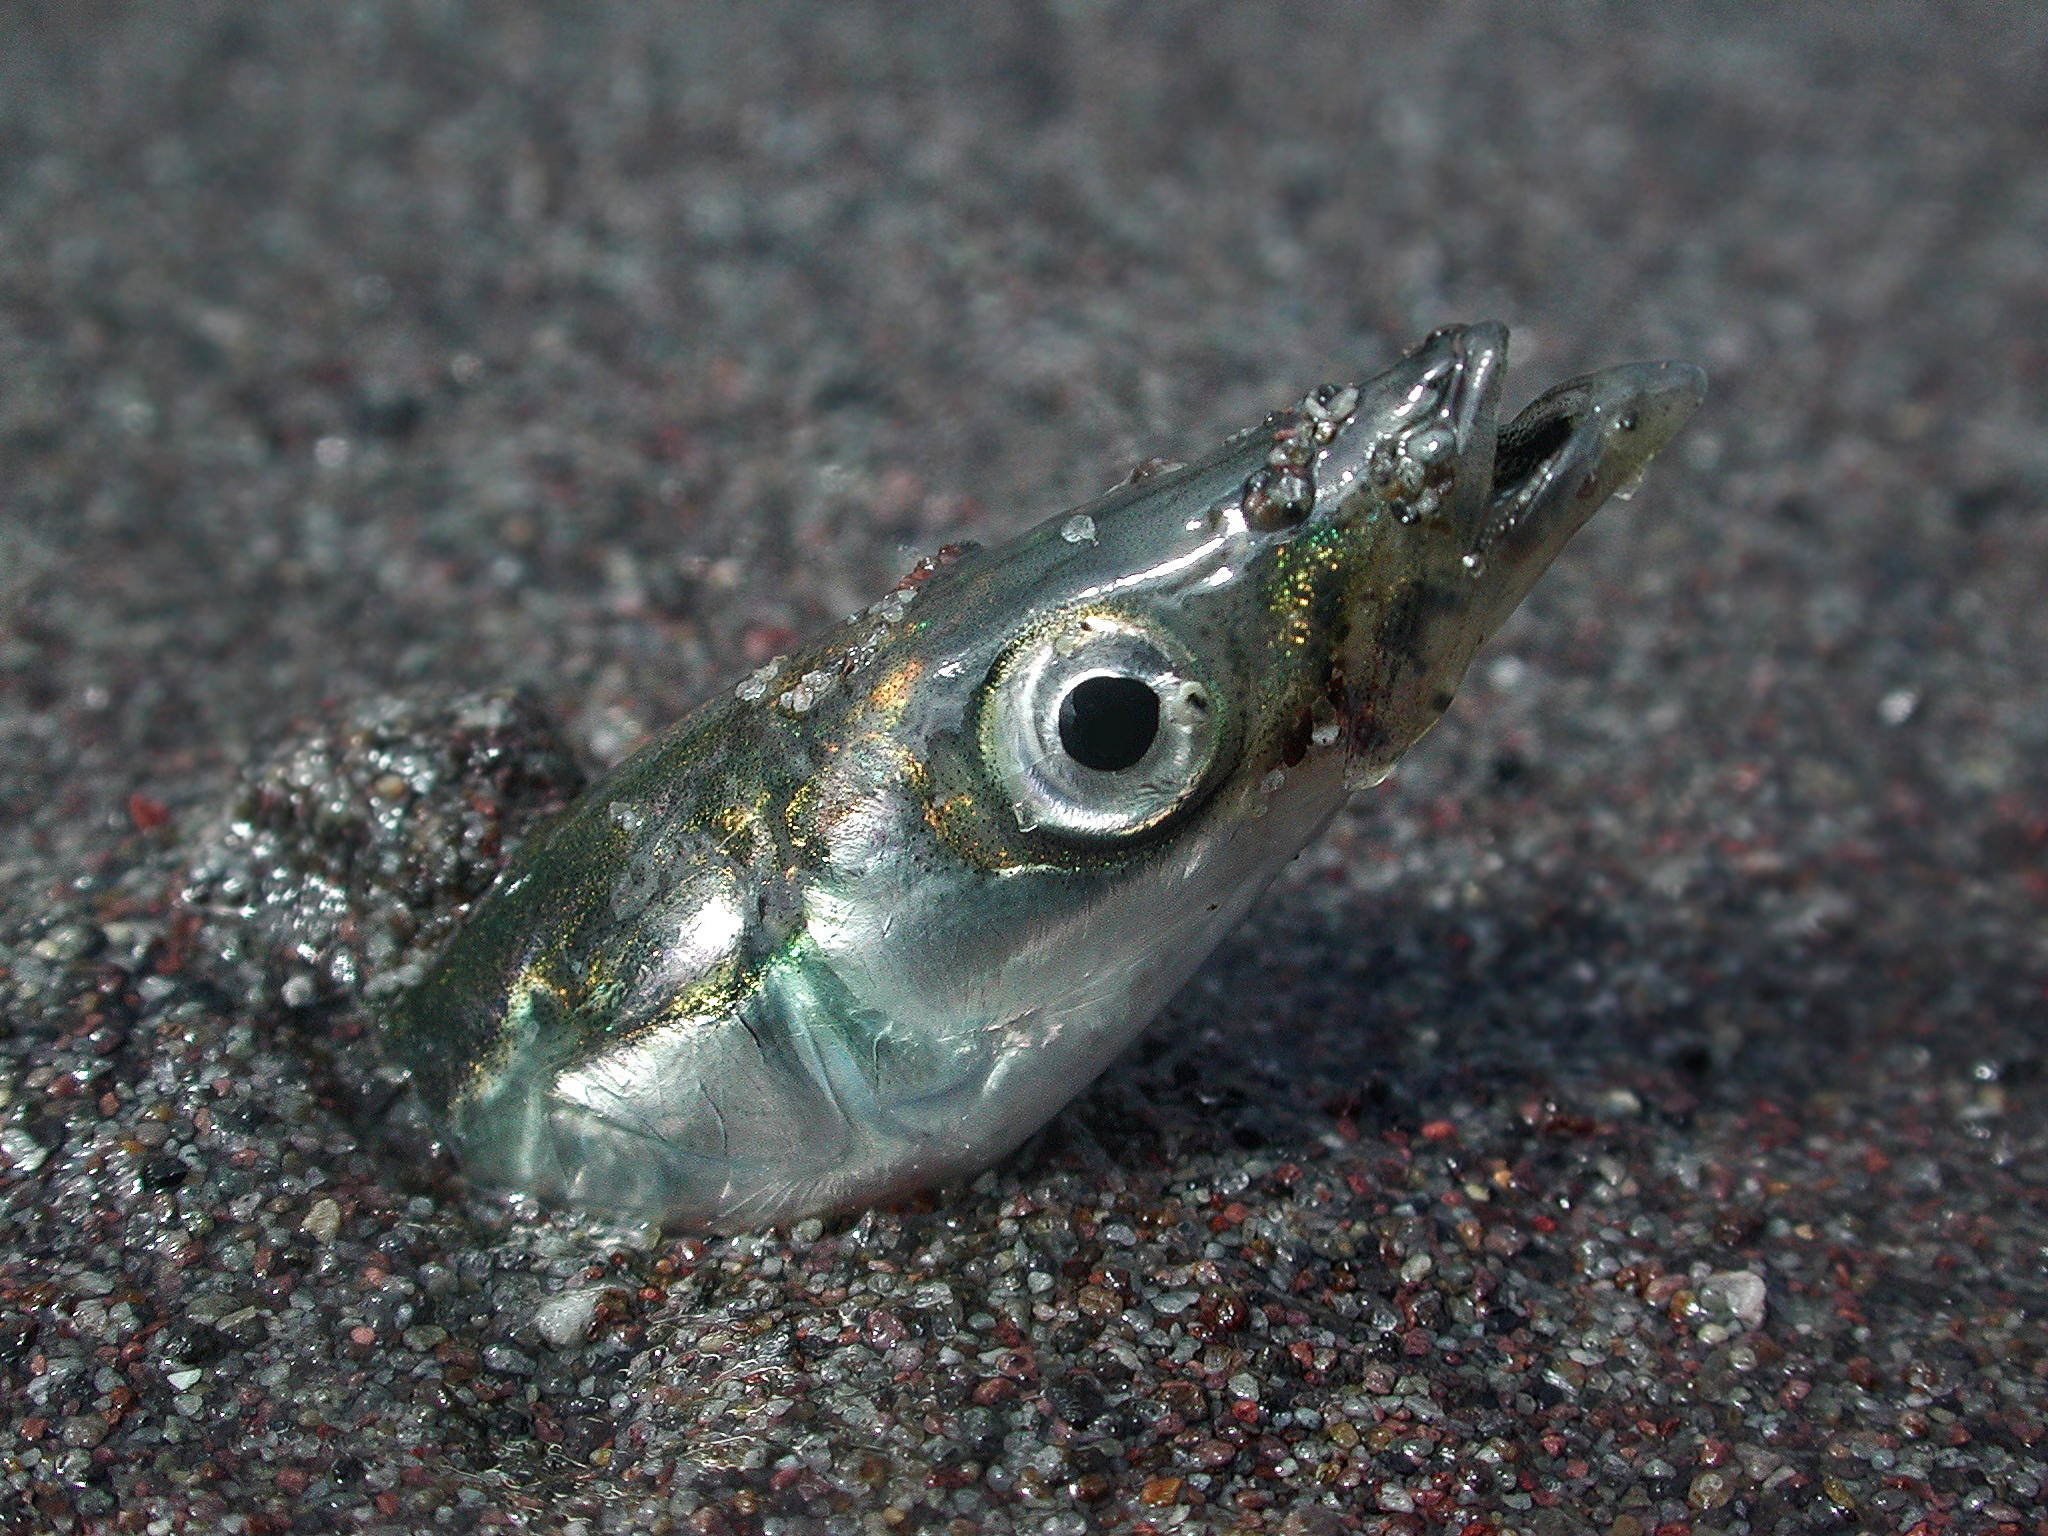
\includegraphics[width=0.5\textwidth]{figures/Ammodytes_hexapterus.jpg} 

        \caption[Sandeel]{A sandeel buried in the sand.}
        \medskip 
        \hspace*{15pt}\hbox{\scriptsize Credit: Original image by Mandy Lindeberg\cite{sandeel_image}}
        \label{sandeel_image}
    \end{figure}

\section{IMRs Acoustic Trawl Surveys}
    When fisheries conduct acoustic surveys of fish, they use \textit{echo sounders} to detect and observe targets in the water remotely. Echo sounders are a special variety of \textit{sonar}, where the acoustic beam produced by a \textit{transducer} is directed vertically downwards from the measuring platform at a set frequency\cite{simmonds2008fisheries}. \gls{imr}s acoustic trawl surveys combine acoustic data from echo sounders, and biological data from trawl catches. The echo sounders in use by the \gls{imr} usually capture acoustic data at multiple frequencies in parallel to maximize the information acquired\cite{korneliussen2018acoustic}. The scrutiny of the data is done through the use of a post-processing software called \gls{lsss}, where \textit{acoustic target classification} is done \textit{manually} with the biological samples as aid\cite{korneliussen2006large}. Afterward, the output \gls{lsss}-data and biological samples are further processed to estimate the fish abundance and age distribution to support \gls{ices} advice\cite{johnsen2019stox}. 

    %Afterwards, the output \gls{lsss}-data and biological samples are input to a software called StoX.  This is an open-source software which is used to estimate the fish abundance and age distribution to be further used as support for \gls{ices} advice\cite{johnsen2019stox}. 
    
    %The echogram for each frequency channel used is stored as a 2-dimensional picture, where each pixel value is a \gls{sv} value.

    
 %Some fish species could not be distinguished from the sprat in the acoustic signal, and more echosounders could have given additional information about the species present\cite{korneliussen2008proposals}. 
        
        %Larger research vessels create a layer of noise consisting of turbulence and bubbles in the water, which can be detrimental to the performance of the echosounder\cite{korneliussen2008proposals}. Hence, the transducers are usually mounted on retractable keels to get below this layer, and as a consequence, vessels usually applied in this context have an 8-meter acoustic  blind zone. The kayak produces significantly less noise in the water, and the retractable keel was only 1.5 meters, and results showed that the vessel managed to measure fish that usually live closer to the surface. In addition, the kayak is less prone to scare away the fish. The lightweight kayak platform enabled it to collect data from shallower water, inaccessible to the larger vessels. However, 

\section{Acoustic Classification of Sandeel} \label{acoustic classification sandeel}

    Acoustic target classification is a significant challenge in most acoustic surveys, and the sandeel is known to be difficult to interpret\cite{sizedependentfreqrespons2009johnsen,johnsen2017collective}.  The earlier mentioned Norwegian sandeel surveys use the \textit{200kHz} frequency to delineate schools, while the \textit{18kHz} and \textit{38kHz} are the most important frequencies for classification when measurements were taken at \textit{18kHz}, \textit{38kHz}, \textit{120kHz}, and \textit{200kHz}\cite{sizedependentfreqrespons2009johnsen}. Some earlier works have had trouble identifying sandeel at \textit{38kHz} and \textit{120kHz}\cite{hassel2004influence,mackinson2005using,mosteiro2004dual}, while some have had success using combinations of the four frequencies \textit{18kHz, 38kHz, 120kHz, and 200kHz} to specifically separate sandeel from herring and mackerel\cite{mohammed2006acoustic}. 

    %It has been shown that large schools of sandeel likely have a connection to the seabed, resulting in severe underestimates of such schools by conventional echosounders\cite{johnsen2017collective}.

    \citet{brautaset2020acoustic} successfully applied deep learning methods to automatically classify sandeel in multi-frequency  acoustic data from the Norwegian sandeel surveys. They extracted and utilized the four frequencies \textit{18kHz}, \textit{38kHz}, \textit{120kHz}, and \textit{200kHz} from the original data, but a problem within deep learning is that feature importance can be difficult to interpret. Hence, it is hard to establish precisely what frequencies contributed the most to their results.
    
    %The objective of this thesis is to create scientific advice for   which echo sounders to be installed on lightweight unmanned vessels, with the goal to classify sandeel in the acoustic data. As mentioned in the previous section, they may have reduced carrying capacity for echo sounders, and the choice of which to install to maximize the information collected is essential. To achieve this, we will expand upon the work of \citeauthor{brautaset2020acoustic} and measure the information stored in all possible subsets of the frequencies contained in the original data from the Norwegian sandeel surveys in the year 2018 and 2019: \textit{18kHz}, \textit{38kHz}, \textit{70kHz}, \textit{120kHz}, \textit{200kHz}, and \textit{333kHz}.

    %Which frequency/frequencies should be used when classifying sandeel in acoustic data, especially if a lightweight vessel, which can only carry a subset of echosounders used during the Norwegian sandeel surveys, are to be equipped to solve the same task? Recently, \citeauthor{brautaset2020acoustic} applied deep learning methods to successfully classify sandeel in acoustic data from these surveys. With this work as a basis, we will investigate the six frequencies \textit{18kHz}, \textit{38kHz}, \textit{120kHz}, \textit{70kHz}, \textit{200kHz}, and \textit{333kHz}, to find which subsets of these are the most informative when classifying sandeel.
%\subsection{Noise}
    %Noise in acoustic data are split into two categories, either \textit{unwanted  targets} produced by the echosounder or signals already present in the medium. The first is defined by the \textit{goal} behind the observation. If we want to observe fish, then plankton is unwanted and vice versa. The latter source of noise originates from either physical (wind, waves...), biological (animals sounds...), or artificial (noise generated by the vessel). By using noise-filtering and 
    
%\subsection{Operatin frequency} ???
    
    
    %\citet{simmonds2008fisheries}
%\subsection{Acoustic data}


%- etter å ha skrevet om SV kan jeg beskrive hvordan dette blir pixlene i bildene fra LSSS.



%\subsection{Echograms and Image Data} \label{echosounder and image data acoustic }
   %% Forsøk 2
   %Echograms represent some visible observation of the water column below the echosounder, and measuring the backscatter of several frequencies channels in parallel, each frequency channel can be viewed as similar to color channels in a picture\cite{brautaset2020acoustic}. Hence, machine learning techniques usually applied to image data are also applicable to \textit{echograms}. Figure \ref{accoustic data and color channels fig} illustrates an example of this:

    %% Forsøk 1
    %This section describes the data gathered by the Simrad EK60 echosounder system produced during the yearly acoustic trawl surveys conducted by the \gls{imr}\cite{johnsen2017collective} and how it relates to image data. Echosounders are maritime instruments, in this case mounted below a ship, which emit acoustic waves into the water (\textit{ping}) and log the backscattered waves\cite{brautaset2020acoustic}. The logs record the \gls{sv}. The data is 2-dimensional, recording the \textit{date and time of the ping} and \textit{range} (\textit{depth}) of the backscattered waves, for each frequency channel used during the measurement. This output is called an \textit{echogram}. As the ping rate was set to 1Hz\cite{choi2021semi}, with a pulse duration of 1.024 milliseconds, the length of each pixel is 1 second horizontally and 19.2 centimeters vertically. These echograms represent some visible observation of the water column below the echosounder, and because of this, each frequency channel can be viewed as similar to color channels in a picture. Hence, machine learning techniques usually applied to image data are also applicable to \textit{echograms}. Figure \ref{accoustic data and color channels fig} illustrates an example of this:
    
    %% NYTT FORSØK
    %This section describes the data gathered by the Simrad EK60 echosounder system produced during the yearly acoustic trawl surveys conducted by the \gls{imr}\cite{johnsen2017collective} and how it relates to image data. Using six frequencies simultaneously to produce pings, they generated multidimensional echograms where each channel is the \gls{sv} values for each frequency. Hence, each frequency channel can be viewed as similar to the color channels in a picture, as these are similarly, varying representations of the same observations. Figure \ref{accoustic data and color channels fig} illustrates an example of this:
    
    % HER ELLER OVER ER DEN JEG VIL BRUKE
    %This section describes the data gathered by the Simrad EK60 echosounder system produced during the yearly acoustic trawl surveys conducted by the \gls{imr}\cite{johnsen2017collective} and how it relates to image data. Using six frequencies simultaneously to produce pings, they generated multidimensional echograms where each channel is the \gls{sv} values for each frequency. Hence, each frequency channel can be viewed as similar to the color channels in a picture, as these are similarly, varying representations of the same observations. Figure \ref{accoustic data and color channels fig} illustrates an example of this:
    
    %The data is 2-dimensional, recording the \textit{date and time of the ping} and \textit{range} (\textit{depth}) of the backscattered waves, for each frequency channel used during the measurement. This output is called an \textit{echogram}. As the ping rate was set to 1Hz\cite{choi2021semi}, with a pulse duration of 1.024 milliseconds, the length of each pixel is 1 second horizontally and 19.2 centimeters vertically. These echograms represent some visible observation of the water column below the echosounder, and because of this, each frequency channel can be viewed as similar to color channels in a picture. Hence, machine learning techniques usually applied to image data are also applicable to \textit{echograms}. Figure \ref{accoustic data and color channels fig} illustrates an example of this:
    
    %\cite{choi2021semi}
    % Forsøk 3
    %This section describes how the data from multifrequency echoosounders translates to image data\cite{brautaset2020acoustic}. These produces pings using several frequencies simultaneously, each capturing different information about the water column beneath the transducer. Hence, each frequency channel can be viewed as similar to color channels in a picture, as these are similarly, varying representations of the same observations. 
    
    %This section describes how echograms relates to image data. Echosounders are maritime instruments, in this case mounted below a ship, which emit acoustic waves into the water (\textit{ping}) and log the backscattered waves. The logs record the \gls{sv}. With the use of   As the ping rate was set to 1Hz\cite{choi2021semi}, with a pulse duration of 1.024 milliseconds, the length of each pixel is 1 second horizontally and 19.2 centimeters vertically. These echograms represent some visible observation of the water column below the echosounder, and because of this, each frequency channel can be viewed as similar to color channels in a picture. Hence, machine learning techniques usually applied to image data are also applicable to \textit{echograms}. Figure \ref{accoustic data and color channels fig} illustrates an example of this:
    
    % - produced by LSSS
    
   % \begin{figure}[H]
       % \centering
       % 
       % \subfloat[Frequency channels that form an echogram. This example show an example %\gls{sv} data crop with six frequencies, on the log scale.]{
       % 	\includesvg[inkscapelatex=false,width=0.4\textwidth,keepaspectratio]{figures/freq_%stacked.svg}}
       % 	%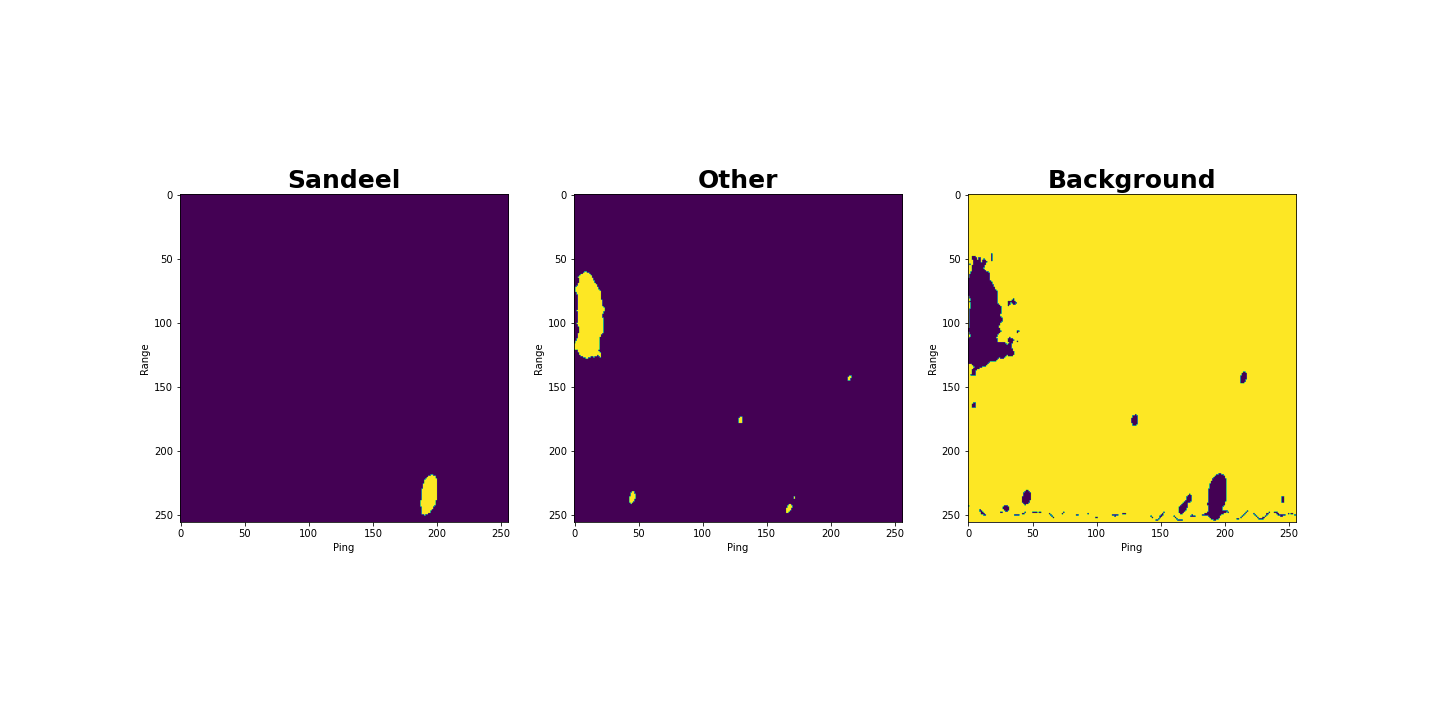
\includegraphics[width=1\textwidth]{figures/data_sample.png} } 
       % 
       % \subfloat[Color channels RGB that forms a picture.]{
       % 	\includesvg[inkscapelatex=false,width=0.9\textwidth,keepaspectratio]{figures/color%s_and_OG.svg}}
       % 
       % 
       % \caption[Frequency channels and color channels]{(a) and (b) both consist of several %channels that together represent some visual observation. \textbf{Credit:} Charles J. %Sharp, CC BY-SA 4.0 <https://creativecommons.org/licenses/by-sa/4.0>, via Wikimedia %Commons}
       % \label{accoustic data and color channels fig}
       % 
       % \end{figure}
    
    %More information about the acoustic data used in this thesis is contained in section %\ref{unet_paper_acoustic}. 
    
    

    
    
    %\citeauthor{brautaset2020acoustic}
    
    
    
    %This thesis goal is to find the subset of frequencies that capture most information to correctly classify the sandeel, and will perform the analysis through the use of \textit{deep learning}, a field within \textit{machine learning} and investigate the six frequencies \textit{18kHz}, \textit{38kHz}, \textit{120kHz}, \textit{70kHz}, \textit{200kHz}, and \textit{333kHz}.
    
    
    
    %using \gls{sv}

%The sandeels lack of swim bladder gives it a low \gls{ts}, and a swimming pattern that is usually not horizontal, which causes problems as the angle of the fish can change the backscattered signal\cite{Forland2014Broadbandwidth}.

%Greenstreet





    % Advisory work, and acoustic trawls
    
    % Acoustic data, applications of machine learning techniques, where a sucessfull approach has been CNN, is similar to image data in. 
    
    % 

%    The Norwegian \gls{imr} is owned by the Ministry of Fisheries and Coastal Affairs, and %its role is to perform research and act as an advisory service in questions surrounding %marine ecosystems and aquaculture\cite{IMR}. Fishing quotas is one such advisory task and %includes the gathering of large amounts of acoustic data. This data is collected by %research vessels\cite{IMR-vessels} equipped with an array of up to six echosounders, %research equipment, trawl equipment and facilities for the crew. This quickly becomes an %expensive endeavour and now the \gls{imr} is looking into alternative solutions to %acquire the same data. 
%    
%    Lightweight autonomous drones\cite{johnsen2020measuring} has been tested in Årdalsfjorden %and involved a kayak with an electric motor and only one 200kHz echosounder installed. %The drone were enabled for autonomous behavior as well as direct remote control. Results %showed that the drone were able to measure fish that usually live closer to the surface %in the acoustic 8-meter blind zone of the larger vessels, as the echosounders are %installed on the bottom part of the research ship. In addition, the drone produces %significantly less noise in the water and are less prone to scare away the fish. The %lightweight platform enabled the kayak-drone to collect data from shallower water, %earlier inaccessible to the larger vessels. The end result was a success for the %kayak-drone, but the manned vessels are still needed for the biological samples in %addition to the acoustic data. 
    
    %\section{Difference picture and acoustic data}
%\todo{DO THIS}
    

    %\textbf{\gls{cv}} is a very popular field of research within deep learning\cite{voulodimos2018deep_computer_vision}. This is because it has mainly focused on tasks we humans do seemingly without training, while computers struggle with it. Examples are facial recognition and object detection in video and image data. There are also works that have gone beyond human capability, like \citeauthor{davis2014visual_deep_video_audio}s\cite{davis2014visual_deep_video_audio} work, where they recovered sounds from the vibrations they induced in objects captured on video. 
    
\section{Unmanned Vehicles in Marine Science} \label{Unmanned Vehicles in Marine Science}
        In \citeyear{VERFUSS201917} \citeauthor{VERFUSS201917}\cite{VERFUSS201917} reviewed the current status of unmanned vehicles suitable for monitoring marine life. The different types of vehicles can operate stationary or moving, on the ocean surface, as aerial or submerged.  They can either be remotely controlled, autonomous, or a combination of both. Unmanned vehicles can use a wide array of sensors, but will often have restrictions on what sensors it can carry. For example, the number or types of transducers installed on acoustic platforms can quickly become a weight problem as the weight of a transducer drastically increases at lower frequencies\footnote{Two sample transducers sold by Kongsberg Maritime for fisheries at the frequencies 18kHz and 333kHz weigh respectively 85kg and 2kg \cite{kongsberg_transducers}.}. Many of the vessels reviewed are commercially available, which has led to a growth in number and use.  The increase in unmanned vehicles and the possibility of gathering more complex data will lead to an exponential rise in the data collected in marine science\cite{malde2020machine}. This further increases the need to make automated programs, or better tools to aid in the current manual data processing, which today is a major chokepoint. Furthermore, the nature of the data gathered will change, possibly in decreasing quality, as humans will have fewer or no opportunities to actively engage in the autonomous information gathering processes.
        %Possibly, further increasing the need for more support vessels and personnel with expertise system knowledge.
        
        %They can use a wide array of sensors, but in the case of acoustic sensors, \citeauthor{VERFUSS201917} emphasized the need to efficiently assign the correct species to the measured animal. This directly impacts the technical requirements of the vehicles purchased, as they need a minimum amount of information provided by the sensors to solve the given task.
        
        During the summer of \citeyear{johnsen2020measuring}, an unmanned vessel was tested in Årdalsfjorden in Norway and involved a kayak with an electric motor, and one 200kHz echosounder was installed to measure \textit{sprat} abundance. Earlier surveys had indicated that large numbers of sprat lives close to the surface, in which the traditional research vessels have an acoustic blind zone\footnote{Echosounder are usually mounted on the bottom of the vessel, creating a blind zone up to the surface. Often on a retractable keel to get underneath a layer of bubbles that can be detrimental to the echosounders performance \cite{korneliussen2008proposals}.}. The kayak survey showed that the small vessel managed to measure high densities of sprat in the blind zone. It was also less prone to scare away the fish as the kayak produced significantly less noise, and its size allowed access to shallower waters. The result was positive for the continued use of unmanned vessels, but the manned vessels are still needed for biological samples\cite{johnsen2020measuring}.
        


\section{Research Question}
        This thesis aims to create scientific advice on which echo sounders to be installed on lightweight unmanned vessels, intending to classify sandeel in the acoustic data. They may have reduced carrying capacity or other limitations for echo sounders, and the choice of which to install to maximize the information collected is essential. To achieve this, we will expand upon the work of \citeauthor{brautaset2020acoustic} and measure the information stored in all possible subsets of the frequencies contained in the original data from the Norwegian sandeel surveys in the year 2018 and 2019: \textit{18kHz}, \textit{38kHz}, \textit{70kHz}, \textit{120kHz}, \textit{200kHz}, and \textit{333kHz}. The research question is stated as follows:
        
        
    \begin{itemize}
        \item \textbf{As lightweight vessels may not have the capacity to carry all the six echo sounders the \gls{imr} usually deploys on the Norwegian sandeel surveys, which ones should be prioritized when classifying sandeel in multi-frequency acoustic data?}
        
        %My work will use data focused around sand eel, hence the results for other species will most likely differ.
        %\item Mulige:
        %\item Kan man trene en model med god ytelse ved å bruke pseudo labels fra en annen model?
        %\item 
    \end{itemize}


\section{Chapter Overview}
    This section describes the outline of the thesis and, in short, the content of each chapter.
    \begin{itemize}
        \item \textbf{Chapter 2 - Background: } Describes the concepts used in this thesis. First marine acoustics in section \ref{acoustics}, then machine learning and artificial neural networks in the following sections.
        \item \textbf{Chapter 3 - Basis and related work:} Describes the basis work for which this thesis seeks to further expand upon in section \ref{unet_paper_acoustic}, and details more recent related research in section \ref{related_work}.
        \item \textbf{Chapter 4 - Material and Methods:} Describes the approach to answering the research question. First, our data and the tools utilized, then how the labels were produced combined with data generation, and finally, our experiment.
        \item \textbf{Chapter 5 - Results:} Describes the results from the experiment, which starts with an evaluation of the training process. Then the results are summarized, followed by different findings in the results for our analysis. 
        \item \textbf{Chapter 6 - Discussion:}  Analyses the results and discuss their implication. 
        \item \textbf{Chapter 7 - Conclusion and Future Work:}  Describes the answer to the research question, summarizes key findings, and states recommendations for future work.
    \end{itemize}

%You can do listings, like in Listing~\ref{ListingReference}
%\begin{lstlisting}[caption={[Short caption]Look at this cool listing. Find the rest in %Appendix~\ref{Listing}},label=ListingReference]
%$ java -jar myAwesomeCode.jar
%\end{lstlisting}

%You can also do language highlighting for instance with Golang:
%And in line~\ref{LineThatDoesSomething} of Listing~\ref{ListingGolang} you can see that we can ref to lines in listings.

%\begin{lstlisting}[caption={Hello world in Golang},label=ListingGolang,escapechar=|]
%package main

%import "fmt"

%func main() {
%    fmt.Println("hello world") |\label{LineThatDoesSomething}|
%}

%\end{lstlisting}



%Example of a centred figure
%\begin{figure}[H]
%    \centering
%    \includegraphics[scale=0.5]{figures/Flowchart}
%    \caption{Caption for flowchart}
%  	\medskip 
%	\hspace*{15pt}\hbox{\scriptsize Credit: Acme company makes everything %\url{https://acme.com/}}
%    \label{FlowchartFigure}
%\end{figure}



